\chapter{Metodi basati sul gradiente}
I problemi di  ottimizzazione si applicano a problemi NLP non vincolati e con una funzione obiettivo differenziabile. Può essere scritto come:
\begin{equation}
    \min_{x \in \mathbb{R}^n} f(x)
\end{equation}
dove $f: \mathbb{R}^n \rightarrow \mathbb{R}$ è una funzione differenziabile, e anche $f \in C^1(R^n)$\\
Sono metodi iterativi che, a partire da un punto iniziale $x^{(k)} \in R^n$, generano una successione di vettori $\{ x^{(k)} \}_{k \in \mathbb{N}} \subset \mathbb{R}^n$.
I metodi che studieremo fanno parte della classe dei \textbf{metodi di discesa}, ossia hanno le proprietà
$$
f\big(x^{(k+1)}\big) < f\big(x^{(k)}\big), \quad k = 0, 1, \dots
$$
Essenzialmente nel costruire la nuova approssimazione, la funzione obbiettivo nella nuova approssimazione assume un valore inferiore rispetto al valore che la funzione obbiettivo assume nell'approssimazione precedente.

Quando si descrive un metodi iterativo bisogna specificare la regola per passare dall'iterazione precedente a quella successiva (questo è solo uno dei tanti aspetti di questi metodi), la nuova approssimazione può essere ottenuta mediante:
$$
x^{(k+1)} = x^{(k)} + \alpha_k\, d^{(k)}, \quad k = 0, 1, \dots
$$
dove:
\begin{compactitemize}
 \item $d^k \in R^n$ è detta \textbf{direzione di discesa}
 \item $\alpha_k \in R_{>0}$ è detto \textbf{parametro di lunghezza di passo}
\end{compactitemize}

\begin{infobox}[Nota bene]
    Partendo dall'iterato $x^k$, il nuovo punto della succession $x^{k+1}$ si trova muovendosi lungo la direzione di ricerca $d^k$ con uno spostamento determinato dal parametro $\alpha_k$
    \begin{figure}[H]
        \centering
        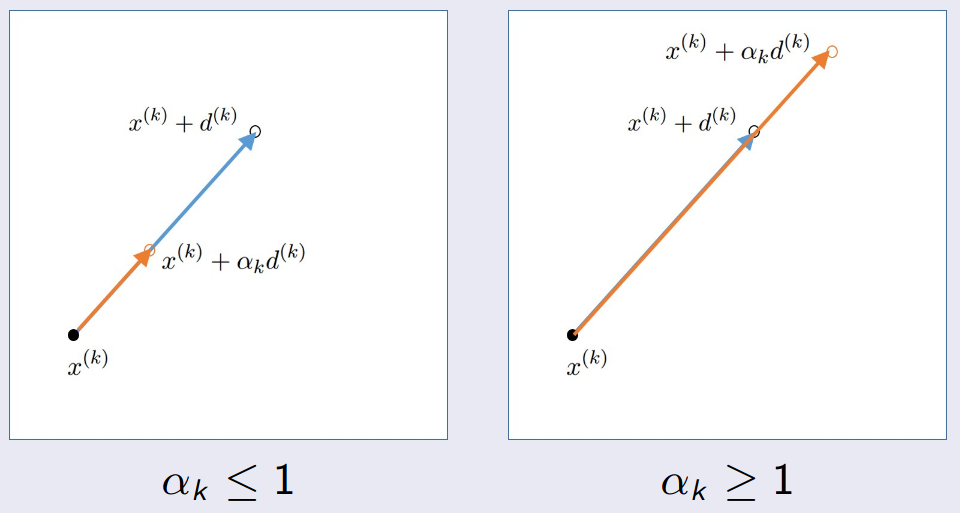
\includegraphics[width=0.6\textwidth]{images/MM1.png}
        \label{fig:cnn_architecture}
    \end{figure}
\end{infobox}

\begin{definizione}[Direzioni di discesa]
    Dato un punto $x \in R^n$, un vettore $d \in R$ che soddisfa la disuguaglianza
    $$
    \nabla f(x)^{T} d < 0
    $$
    viene detto \textbf{direzione di discesa} per $f$ in $x$.
\end{definizione}
\begin{figure}[H]
    \centering
    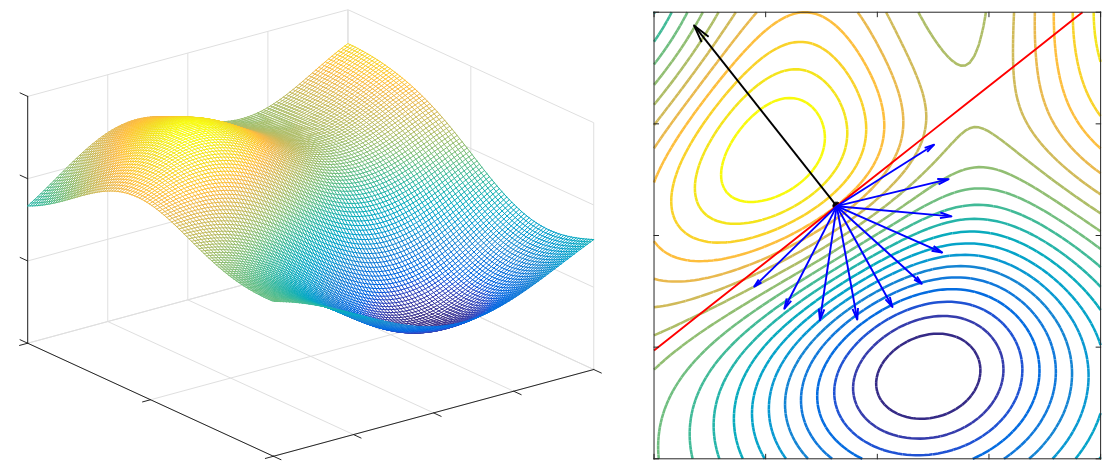
\includegraphics[width=0.7\textwidth]{images/MM2.png}
    \caption{Valori alti corrispondono a colori caldi (giallo), valori bassi a colori freddi (blu).}
    \label{fig:cnn_architecture}
\end{figure}
\textbf{Osservazione (1)}:
Dalla definizione di derivata direzionale per funzioni $C^1$, si ha che
\[
\lim_{\alpha \to 0^+} \frac{f(x + \alpha d) - f(x)}{\alpha} = \nabla f(x)^T d
\]
Se $d$ è una direzione di discesa per $f$ in $x$, dal teorema della permanenza del segno si ha che esiste $\bar{\alpha} > 0$ tale che
\[
\frac{f(x + \alpha d) - f(x)}{\alpha} < 0, \quad \forall \alpha \in (0, \bar{\alpha}] 
\quad \Rightarrow \quad
f(x + \alpha d) < f(x), \quad \forall \alpha \in (0, \bar{\alpha}].
\]

\newpage
\textbf{Osservazione (2)}:  
Sia $x \in \mathbb{R}^n$. Se $x$ non è un punto stazionario per $f$, allora esiste almeno una direzione di discesa per $f$ in $x$.  
Viceversa, se non esistono direzioni di discesa per $f$ in $x$, allora $x$ è un punto stazionario di $f$.

Se $\nabla f(x) \neq 0$, allora
\[
d = -\nabla f(x)
\]
è una direzione di discesa, infatti
\[
\nabla f(x)^T d = - \|\nabla f(x)\|^2 < 0.
\]

Supponiamo invece che 
\[
\nabla f(x)^T d \ge 0, \quad \forall d \in \mathbb{R}^n.
\]  
Fissato $d \in \mathbb{R}^n$, la disuguaglianza vale sia per $d$ che per $-d$:
\[
\nabla f(x)^T d \ge 0, \quad \nabla f(x)^T (-d) \ge 0 \quad \Rightarrow \quad \nabla f(x) = 0.
\]

\begin{algorithm}
    \caption{Metodo di discesa del gradiente con criterio di arresto}
    \begin{algorithmic}[1]
    \State \textbf{Input:} $x^{(0)} \in \mathbb{R}^n$, $\tau > 0$
    \For{$k = 0, 1, 2, \dots$}
        \If{$\|\nabla f(x^{(k)})\| \le \tau$}
            \State \textbf{Stop}
        \Else
            \State \textbf{Step 1:} Calcolare una direzione di discesa $d^{(k)}$ per $f$ in $x^{(k)}$
            \State \textbf{Step 2:} Calcolare $\alpha_k$ tale che
            \[
            f(x^{(k)} + \alpha_k d^{(k)}) < f(x^{(k)})
            \]
            \State \textbf{Step 3:} Calcolare il nuovo punto
            \[
            x^{(k+1)} = x^{(k)} + \alpha_k d^{(k)}
            \]
        \EndIf
    \EndFor
    \end{algorithmic}
\end{algorithm}
I metodi del gradiente si arrestano nei punti stazionari.  
In generale, sotto opportune ipotesi, l’output dei metodi del gradiente è un’approssimazione di un punto stazionario per il problema NLP, ossia di una soluzione del sistema di equazioni non lineari $\nabla f(x) = 0$.
Sotto ipotesi di convessità si può parlare di punti di minimo.

\textbf{Osservazione (3)}:Il criterio di arresto
\[
\|\nabla f(x^{(k)})\| \le \tau
\]
è associato al residuo del problema della ricerca dei punti stazionari della funzione $f$:
\[
\nabla f(x) = 0.
\]

Altri criteri di arresto includono la distanza relativa tra le iterate:
\[
\frac{\|x^{(k+1)} - x^{(k)}\|}{\|x^{(k)}\|} \le \tau,
\]
e la differenza relativa tra i valori della funzione obiettivo:
\[
\frac{f(x^{(k)}) - f(x^{(k+1)})}{f(x^{(k)})} \le \tau.
\]
\begin{figure}[H]
    \centering
    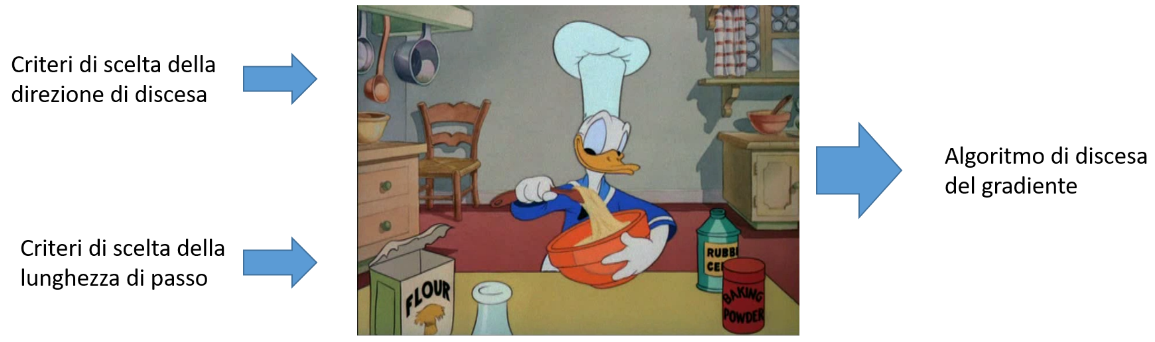
\includegraphics[width=0.7\textwidth]{images/MM3.png}
    \caption{Riassunto per ottenre un algortimo di discesa del gradiente.}
    \label{fig:cnn_architecture}
\end{figure}

\section{Selezione della direzione di discesa}
L'idea è quella di costruire la direzione di discesa seguendo questa regola:
$$
d^{(k)} = -D_k \, \nabla f(x^{(k)})
$$
Essenzialmente prendo l'anti-gradiente (gradiente col meno davanti) e lo pre-moltiplico (lo moltiplico a sinistra) per la matrice $D_k \in R^{nxn}$, che è una matrice simmetrica definita positiva.
$$
\nabla f(x^{(k)})^T d^{(k)} = - \nabla f(x^{(k)})^T D_k \, \nabla f(x^{(k)}) < 0
$$
In questo modo ho la garanzia di avere individuato una direzione di discesa, perché se prendo una matrice definita positiva il prodotto scritto sopra verrà sempre positivo quindi con meno davanti diventa sempre negativo.
A seconda della scelta di $D_k$ corrispondono diversi metodi del gradiente.